\documentclass[11pt,a4paper]{article}

\usepackage[margin=1in]{geometry}
\usepackage[T1]{fontenc}
\usepackage[utf8]{inputenc}
\usepackage{lmodern}
\usepackage{amsmath,amssymb,bm}
\usepackage{graphicx}
\usepackage{booktabs}
\usepackage{array}
\usepackage{caption}
\usepackage{subcaption}
\usepackage{tikz}
\usepackage{hyperref}
\usepackage{xcolor}
\usepackage{listings}

\hypersetup{
    colorlinks=true,
    linkcolor=blue,
    filecolor=magenta,
    urlcolor=blue,
    pdftitle={Motor Thermal FEM Report},
    pdfauthor={Project Report}
}

\title{Thermal Finite Element Analysis of a Slotted Electric Motor Cross-Section\\
\large Physics, Mathematics, Numerical Method, and Results}
\author{Project Technical Report}
\date{\today}

\lstset{
  basicstyle=\ttfamily\small,
  frame=single,
  breaklines=true,
  columns=fullflexible,
  keywordstyle=\color{blue!70!black},
  commentstyle=\color{green!40!black}
}

\begin{document}
\maketitle

\begin{abstract}
This report documents a 2D finite element model for steady-state thermal analysis of an electric motor cross-section. The objective is to solve heat conduction with internal winding losses and convective cooling, while preserving clear physical interpretation and numerical robustness. The model includes: (i) motor-region material partitioning (iron, slot/winding effective medium, air gap), (ii) optional temperature-dependent winding loss, (iii) Robin convective boundaries on both outer stator and inner air-gap sides, and (iv) validation against an analytical annulus benchmark. We summarize the governing physics, derive the weak form, describe the finite element algorithm, and present key simulation results and sensitivity trends.
\end{abstract}

\tableofcontents
\newpage

\section{Problem Overview and Scope}
The project solves two thermal problems:
\begin{enumerate}
    \item \textbf{Phase 1 (verification problem):} A plain annulus with prescribed inner/outer temperatures, compared to analytical solution.
    \item \textbf{Phase 2 (application problem):} A slotted motor cross-section with volumetric winding heating and convective cooling.
\end{enumerate}

The implementation is intentionally transparent: plain Python functions, sparse matrix assembly, and direct sparse solve. The report focus is on physics and mathematics first, then implementation and results.

\subsection*{Modeling assumptions}
\begin{itemize}
    \item Steady state (no transient terms).
    \item Two-dimensional cross-section; results are per unit axial length (W/m).
    \item No radiation term in the base formulation.
    \item Effective material properties are used for slot region and laminated iron approximation.
\end{itemize}

\section{Motor Thermal Physics}
\subsection{Governing equation}
In each material region \(\Omega_m\), the steady heat equation is
\begin{equation}
-\nabla \cdot \left( \mathbf{K}(\mathbf{x},T)\nabla T \right) = q(\mathbf{x},T),
\end{equation}
where \(T\) is temperature, \(\mathbf{K}\) is thermal conductivity (scalar or tensor), and \(q\) is volumetric heat source.

For isotropic regions, \(\mathbf{K}=k\mathbf{I}\). For effective anisotropic iron in polar orientation, a 2\(\times\)2 tensor is used in Cartesian coordinates.

\subsection{Boundary physics}
Two Robin boundaries are used in Phase 2:
\begin{equation}
-\mathbf{n}\cdot(\mathbf{K}\nabla T)=h\left(T-T_{\infty}\right),
\end{equation}
with separate \((h,T_{\infty})\) values for:
\begin{itemize}
    \item Outer stator boundary (external cooling).
    \item Inner air-gap boundary (effective rotor-side cooling).
\end{itemize}

\subsection{Temperature-dependent winding loss}
For winding elements, Joule heating can be updated with temperature:
\begin{equation}
q_{\text{cu}}(T)=q_{\text{ref}}\left[1+\alpha_{\text{cu}}(T-T_{\text{ref}})\right],
\end{equation}
with practical clipping bounds for numerical stability in prototype studies.

\section{Schematics of the Motor Problem}
\subsection{Domain and region schematic}
Figure~\ref{fig:domain-schematic} shows a conceptual cross-section and region partition.

\begin{figure}[h!]
\centering
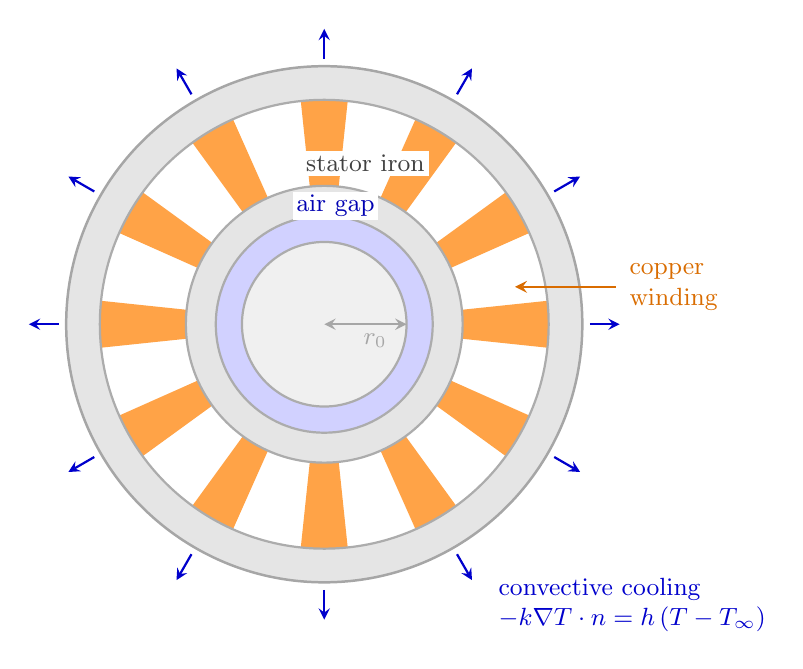
\begin{tikzpicture}[scale=0.95,>=stealth,font=\small]
    % radii (schematic, not to scale)
    \def\rshaft{1.10}
    \def\rgap{1.45}
    \def\rslotin{1.85}
    \def\rslotout{3.00}
    \def\rstator{3.45}

    % region fills
    \fill[gray!20] (0,0) circle (\rstator);   % stator body
    \fill[white]   (0,0) circle (\rslotout);  % ring for slot region
    \fill[gray!20] (0,0) circle (\rslotin);   % inner iron around air-gap
    \fill[blue!18] (0,0) circle (\rgap);      % air gap
    \fill[gray!12] (0,0) circle (\rshaft);    % rotor / shaft

    % copper slot wedges (12)
    \foreach \k in {0,...,11} {
        \pgfmathsetmacro\a{\k*30}
        \fill[orange!72] (\a-6:\rslotin) arc (\a-6:\a+6:\rslotin) --
                          (\a+6:\rslotout) arc (\a+6:\a-6:\rslotout) -- cycle;
    }

    % boundaries
    \draw[line width=0.9pt,gray!70] (0,0) circle (\rstator);
    \draw[line width=0.8pt,gray!65] (0,0) circle (\rslotout);
    \draw[line width=0.8pt,gray!65] (0,0) circle (\rslotin);
    \draw[line width=0.8pt,gray!65] (0,0) circle (\rgap);
    \draw[line width=0.8pt,gray!65] (0,0) circle (\rshaft);

    % outward convection arrows around stator
    \foreach \a in {0,30,...,330} {
        \draw[->,blue!80!black,line width=0.8pt] (\a:3.55) -- (\a:3.95);
    }

    % compact labels
    \node[fill=white,inner sep=1.5pt,text=black!75] at (0.55,2.15) {stator iron};
    \node[fill=white,inner sep=1.2pt,text=blue!70!black] at (0.15,1.58) {air gap};

    % copper winding callout
    \draw[->,orange!85!black,line width=0.9pt] (3.9,0.5) -- (2.55,0.5);
    \node[anchor=west,text=orange!85!black,align=left] at (3.95,0.5) {copper\\winding};

    % radius marker r0
    \draw[<->,line width=0.8pt,gray!70] (0,0) -- (\rshaft,0);
    \node[text=gray!70] at (0.68,-0.22) {$r_0$};

    % convective cooling annotation
    \node[text=blue!80!black,anchor=west,align=left] at (2.2,-3.75)
        {convective cooling\\$-k\nabla T\cdot n = h\,(T-T_{\infty})$};
\end{tikzpicture}
\caption{Schematic of the modeled motor cross-section and thermal boundary conditions.}
\label{fig:domain-schematic}
\end{figure}

\subsection{Heat-flow schematic}
\begin{figure}[h!]
\centering
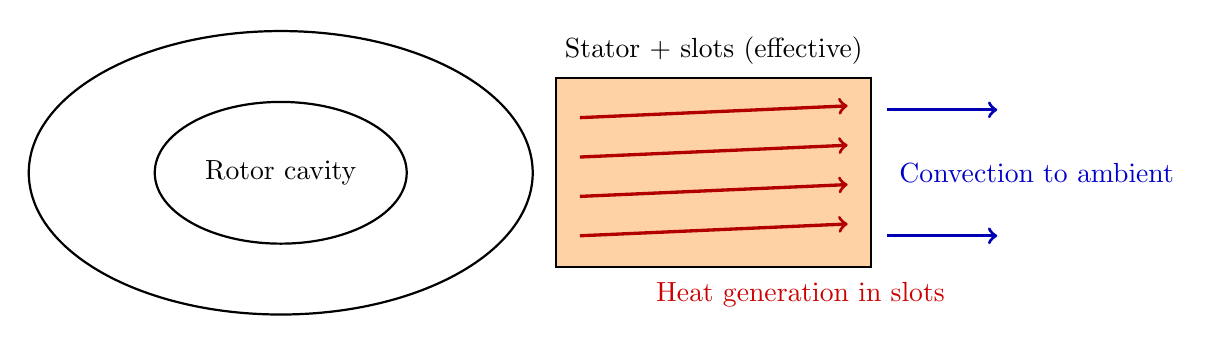
\begin{tikzpicture}[scale=1.0]
    \draw[thick] (-4,0) ellipse (3.2 and 1.8);
    \draw[thick] (-4,0) ellipse (1.6 and 0.9);
    \node at (-4,0) {Rotor cavity};

    \fill[orange!35] (-0.5,-1.2) rectangle (3.5,1.2);
    \draw[thick] (-0.5,-1.2) rectangle (3.5,1.2);
    \node at (1.5,1.55) {Stator + slots (effective)};

    \foreach \y in {-0.8,-0.3,0.2,0.7} {
        \draw[->,very thick,red!70!black] (-0.2,\y) -- (3.2,\y+0.15);
    }
    \node[red!80!black] at (2.6,-1.55) {Heat generation in slots};

    \draw[->,very thick,blue!70!black] (3.7,0.8) -- (5.1,0.8);
    \draw[->,very thick,blue!70!black] (3.7,-0.8) -- (5.1,-0.8);
    \node[blue!80!black] at (5.6,0.0) {Convection to ambient};
\end{tikzpicture}
\caption{Conceptual thermal pathway: winding losses conduct through solids and are removed by convection.}
\label{fig:heat-schematic}
\end{figure}

\clearpage
\section{Finite Element Formulation}
\subsection{Weak form}
Let \(v\) be a test function. Integrating over \(\Omega\) and applying integration by parts gives
\begin{equation}
\int_{\Omega} (\nabla v)^T\mathbf{K}\nabla T\,d\Omega
+ \int_{\Gamma_R} h v T\,d\Gamma
= \int_{\Omega} v q\,d\Omega + \int_{\Gamma_R} h v T_{\infty}\,d\Gamma.
\end{equation}

This leads to linear algebra system
\begin{equation}
\mathbf{K}_g\mathbf{T}=\mathbf{f},
\end{equation}
where \(\mathbf{K}_g\) is sparse and assembled from elemental contributions.

\subsection{Element equations (P1 triangles)}
For linear triangular elements, shape-function gradients are constant inside each element:
\begin{equation}
\nabla N_i = [b_i,\;c_i]^T.
\end{equation}
Element stiffness entries are
\begin{equation}
K_e(i,j)=A_e\,\nabla N_i^T\mathbf{K}_e\nabla N_j.
\end{equation}
Element load entries for uniform source are
\begin{equation}
f_e(i)=q_e A_e/3.
\end{equation}

\subsection{Robin boundary edge contribution}
For a boundary edge of length \(L\):
\begin{equation}
\mathbf{K}_{R,e}=\frac{hL}{6}
\begin{bmatrix}2&1\\1&2\end{bmatrix},
\qquad
\mathbf{f}_{R,e}=\frac{hT_{\infty}L}{2}
\begin{bmatrix}1\\1\end{bmatrix}.
\end{equation}

\subsection{Sparse assembly and solve}
The implementation uses COO triplet accumulation and conversion to CSR format, then direct sparse solve (SuperLU). This is robust for the problem sizes used in this project.

\section{Mesh Strategy and Region Tagging}
\subsection{Phase 1 mesh}
Phase 1 uses a structured annular O-grid with two triangles per logical quadrilateral. This provides smooth refinement and clean convergence studies.

\subsection{Phase 2 mesh}
Phase 2 now uses an interface-conforming structured polar mesh with explicit angular breakpoints at slot boundaries and radial breakpoints at material interfaces. This minimizes interface smearing and avoids centroid-tag ambiguity common in unconstrained triangulation.

\begin{figure}[h!]
    \centering
    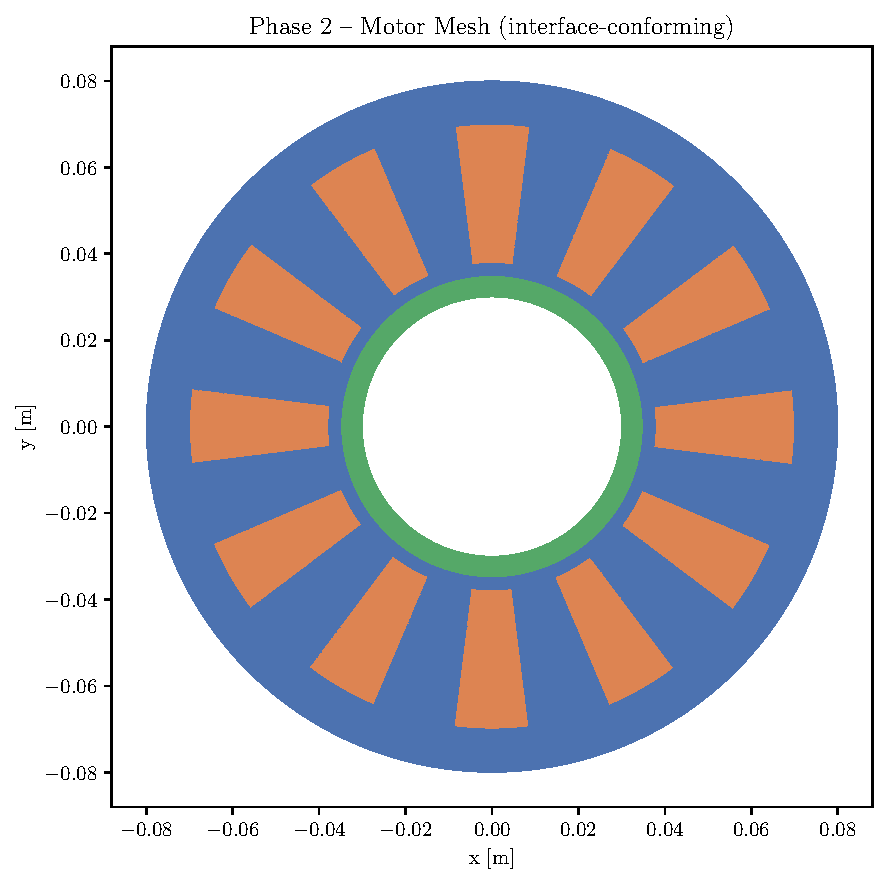
\includegraphics[width=0.62\textwidth]{../results/phase2_mesh.pdf}
    \caption{Generated motor mesh for Phase 2.}
\end{figure}

\section{Algorithm}
\subsection{Overall workflow}
\begin{enumerate}
    \item Build mesh and region tags.
    \item Build per-element conductivity model (tensor in iron, scalar elsewhere).
    \item Initialize volumetric source \(q\) in slots.
    \item Nonlinear fixed-point loop (if \(q(T)\) enabled):
    \begin{enumerate}
        \item Assemble global system including Robin boundaries.
        \item Solve for \(T\).
        \item Update slot \(q(T)\), with under-relaxation and clipping.
        \item Check convergence in \(\Delta T\) and \(\Delta q\).
    \end{enumerate}
    \item Post-process: temperature maps, flux vectors, and energy balance checks.
\end{enumerate}

\subsection{Pseudo-code}
\begin{lstlisting}[language=Python,caption={Simplified Phase 2 solver logic}]
mesh = make_motor_mesh(...)
inner_edges = make_closed_boundary_edges(inner_nodes)
outer_edges = make_closed_boundary_edges(outer_nodes)

q = q_ref in slot elements
for k in range(max_iters):
    K, f = assemble(nodes, elements, conductivity_tensor, q)
    K, f = apply_robin(K, f, outer_edges, h_outer, Tinf_outer)
    K, f = apply_robin(K, f, inner_edges, h_gap, Tinf_gap)
    T = solve(K, f)

    q_new = update_q_from_temperature(T)
    q = (1-omega)*q + omega*q_new
    if converged(T, q):
        break

# final consistency solve with latest q
K, f = assemble(..., q)
T = solve(K, f)
\end{lstlisting}

\clearpage
\section{Results}
\subsection{Phase 1 verification (annulus)}
The annulus benchmark validates implementation quality against analytical solution. Typical run outcomes:
\begin{itemize}
    \item Max pointwise error: \(6.67\times 10^{-3}\,^\circ\mathrm{C}\)
    \item Measured convergence rates: \(L_2\approx1.925\), \(H^1\approx0.983\)
\end{itemize}
These are close to theoretical rates for linear triangular elements (\(O(h^2)\) in \(L_2\), \(O(h)\) in \(H^1\)).

\begin{figure}[h!]
\centering
\begin{subfigure}{0.48\textwidth}
    \centering
    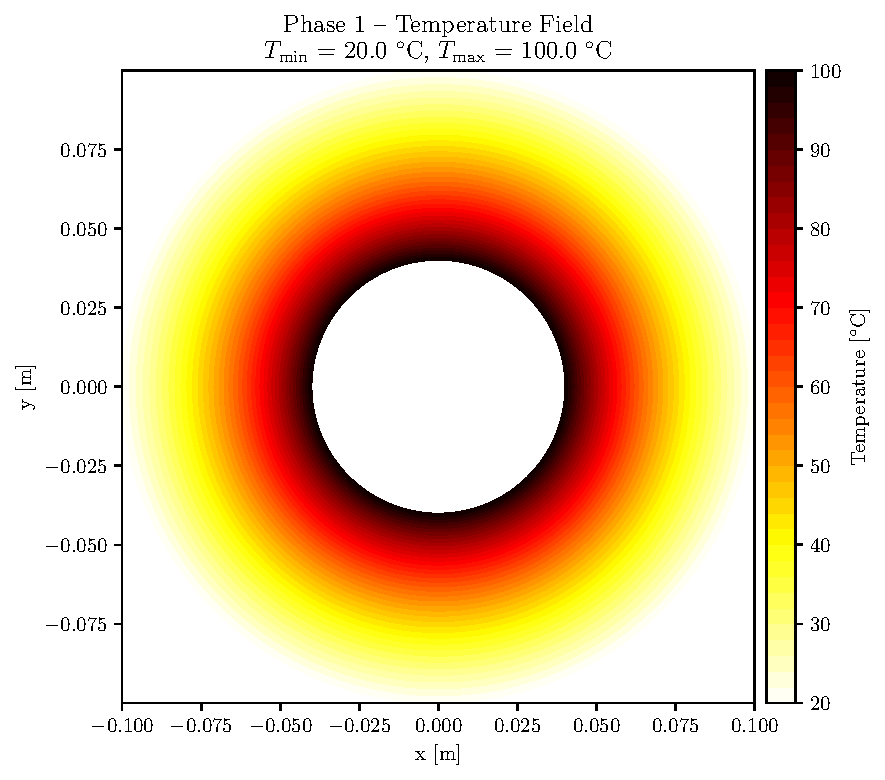
\includegraphics[width=\textwidth]{../results/phase1_temperature.pdf}
    \caption{Phase 1 temperature field}
\end{subfigure}
\hfill
\begin{subfigure}{0.48\textwidth}
    \centering
    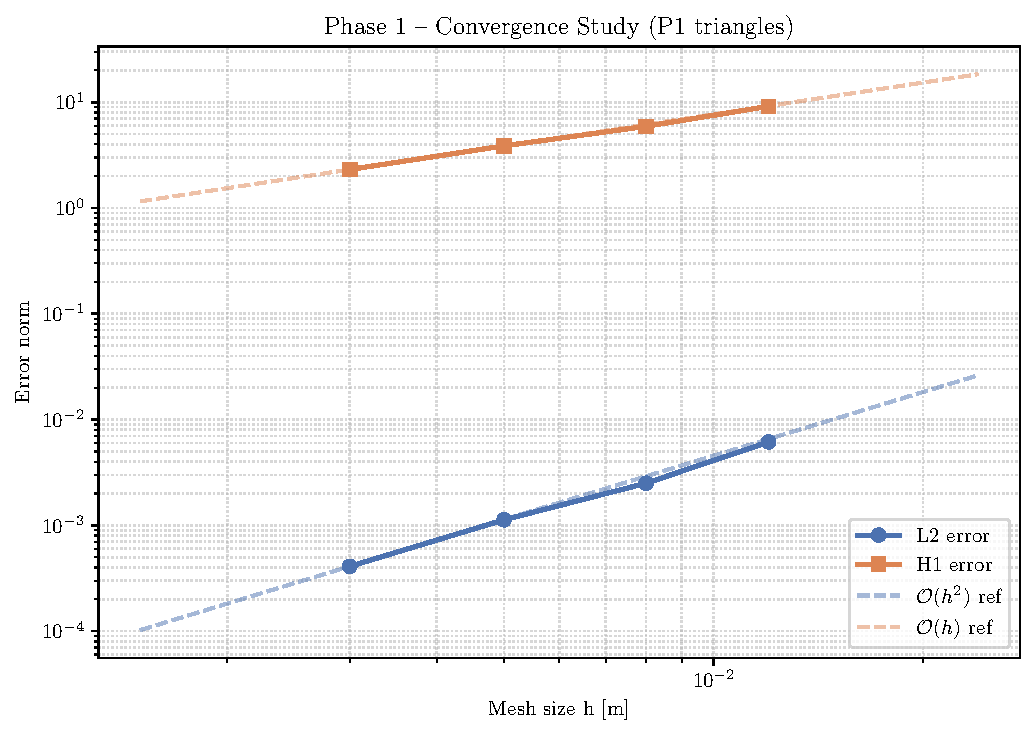
\includegraphics[width=\textwidth]{../results/phase1_convergence.pdf}
    \caption{Phase 1 convergence}
\end{subfigure}
\caption{Verification plots from the annulus benchmark.}
\end{figure}

\subsection{Phase 2 baseline (improved parameter set)}
Using calibrated starter parameters
\(q_{ref}=1.8\times10^6\,\mathrm{W/m^3}\),
\(h_{outer}=180\,\mathrm{W/(m^2K)}\),
\(h_{gap}=120\,\mathrm{W/(m^2K)}\),
\(k_{slot,eff}=5\,\mathrm{W/(mK)}\),
\(k_r=22\), \(k_t=30\),
the model produced:
\begin{itemize}
    \item Peak winding temperature \(\approx 175.5\,^\circ\mathrm{C}\)
    \item Robin energy-balance residual \(\approx 0.0\%\)
    \item Independent conductive boundary check residual \(\approx 1.4\%\)
\end{itemize}

\begin{figure}[h!]
\centering
\begin{subfigure}{0.48\textwidth}
    \centering
    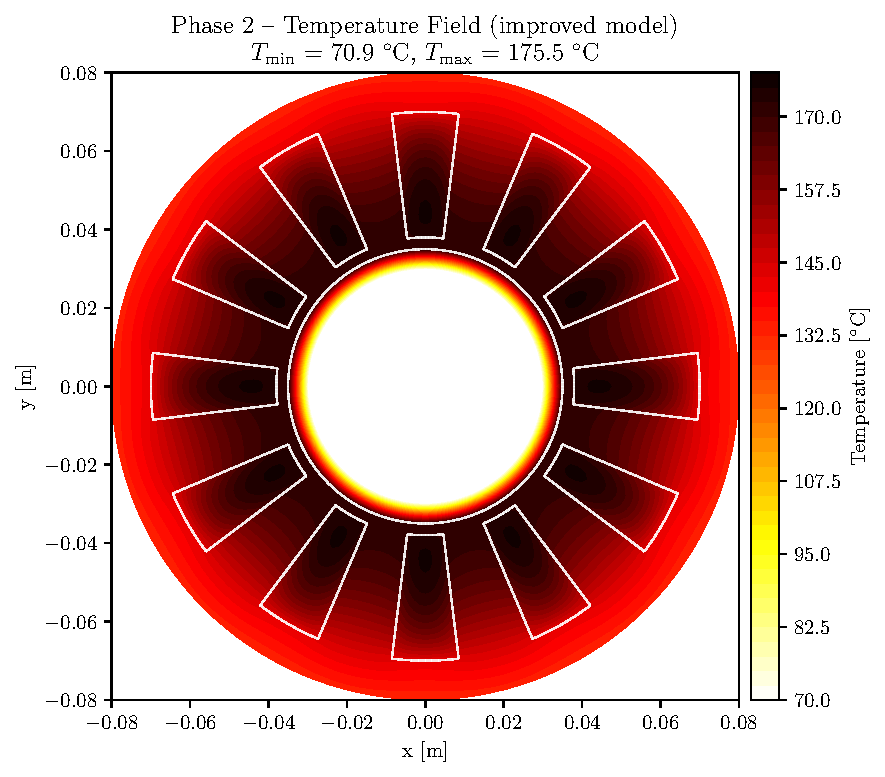
\includegraphics[width=\textwidth]{../results/phase2_temperature.pdf}
    \caption{Baseline temperature field}
\end{subfigure}
\hfill
\begin{subfigure}{0.48\textwidth}
    \centering
    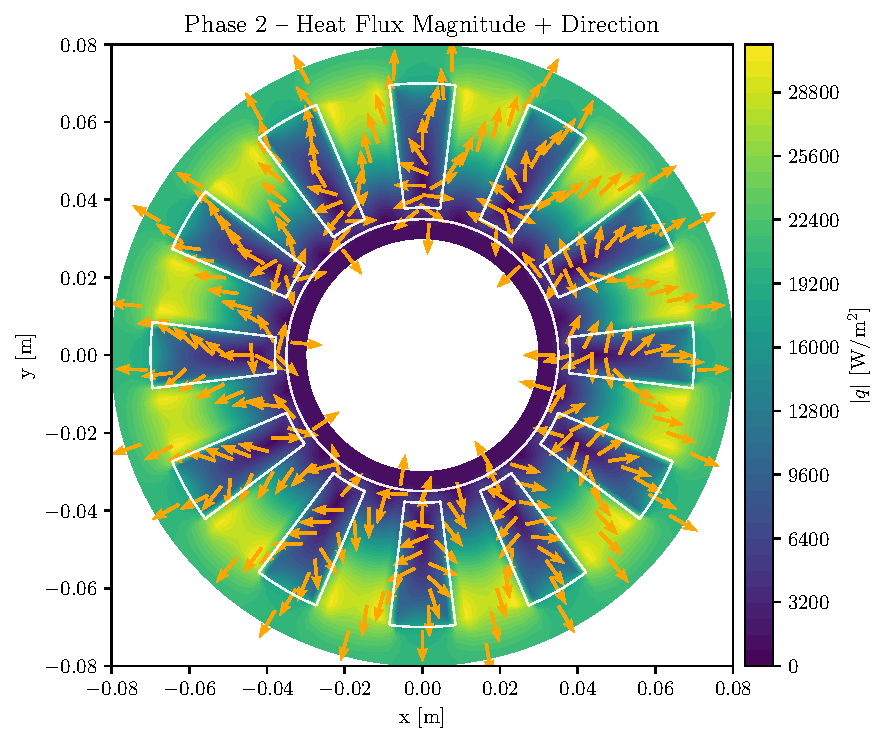
\includegraphics[width=\textwidth]{../results/phase2_heatflux.pdf}
    \caption{Flux magnitude and direction}
\end{subfigure}
\caption{Phase 2 baseline fields.}
\end{figure}

\subsection{Sensitivity trends}
The parametric trends are physically consistent:
\begin{itemize}
    \item \(T_{peak}\) increases with winding heat load.
    \item \(T_{peak}\) decreases with stronger outer convection.
    \item \(T_{peak}\) decreases with higher slot effective conductivity.
\end{itemize}

\begin{figure}[h!]
\centering
\begin{subfigure}{0.32\textwidth}
    \centering
    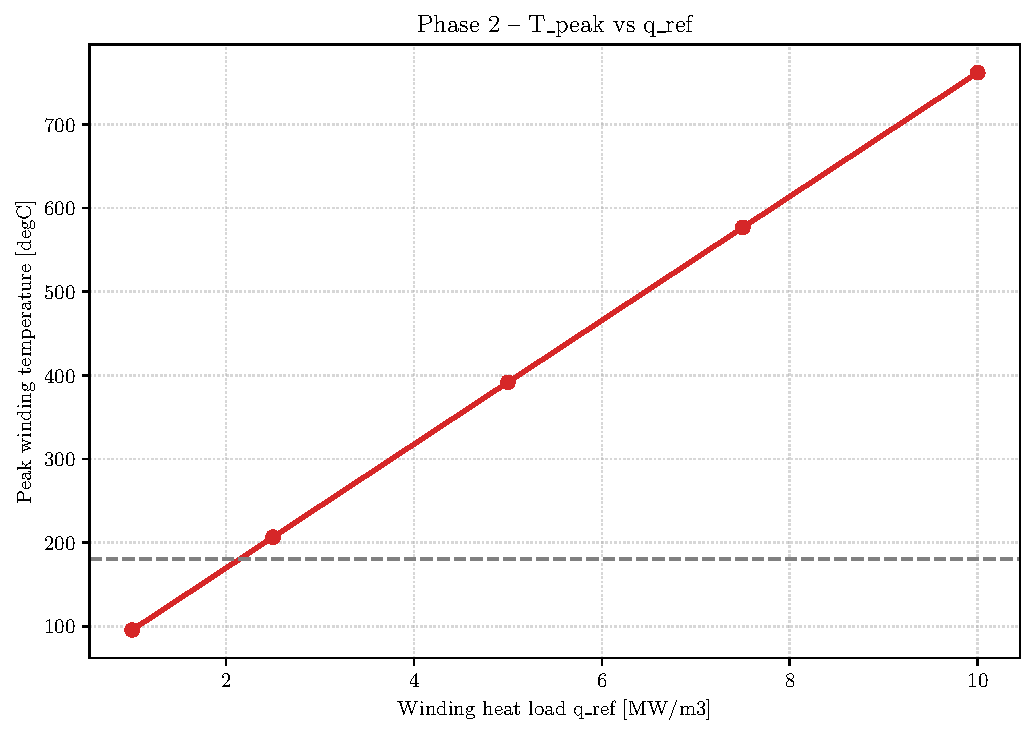
\includegraphics[width=\textwidth]{../results/phase2_parametric.pdf}
    \caption{$T_{peak}$ vs $q_{ref}$}
\end{subfigure}
\hfill
\begin{subfigure}{0.32\textwidth}
    \centering
    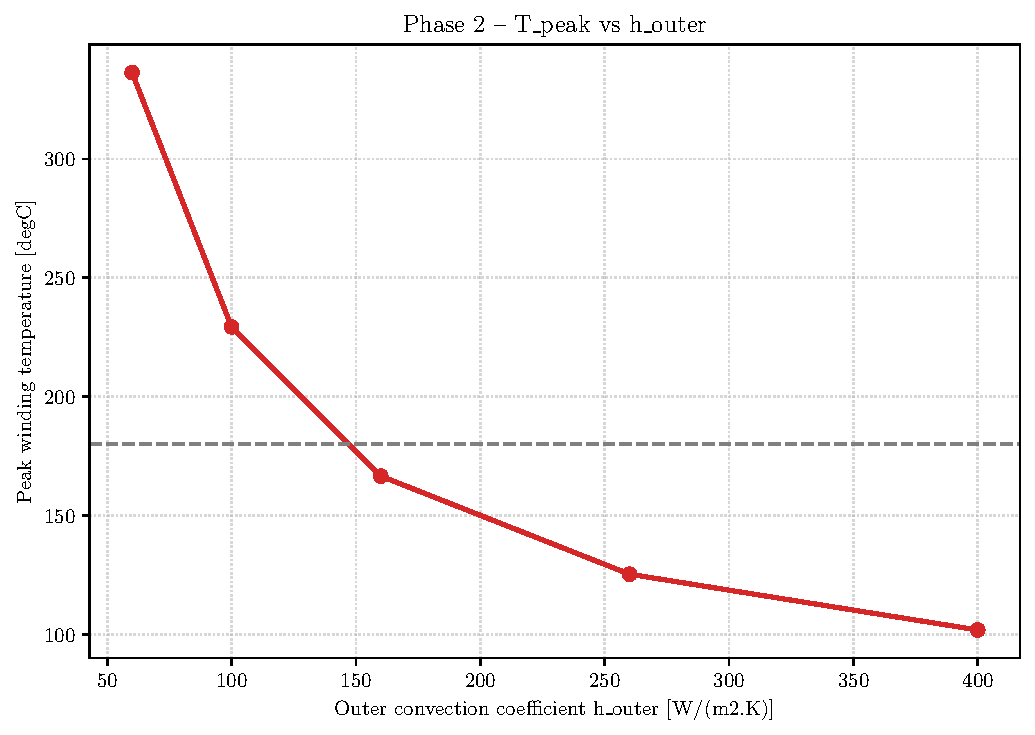
\includegraphics[width=\textwidth]{../results/phase2_parametric_houter.pdf}
    \caption{$T_{peak}$ vs $h_{outer}$}
\end{subfigure}
\hfill
\begin{subfigure}{0.32\textwidth}
    \centering
    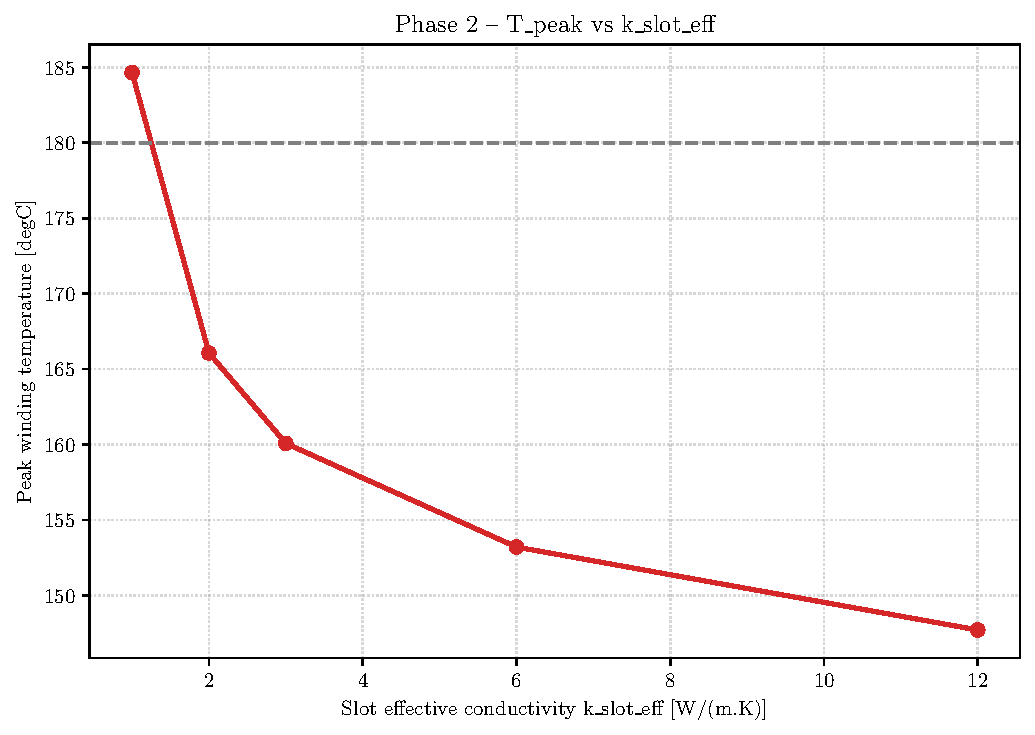
\includegraphics[width=\textwidth]{../results/phase2_parametric_kslot.pdf}
    \caption{$T_{peak}$ vs $k_{slot,eff}$}
\end{subfigure}
\caption{Phase 2 sensitivity studies.}
\end{figure}

\clearpage
\section{Discussion}
\subsection{What is validated}
\begin{itemize}
    \item Mathematical correctness of FEM implementation is supported by Phase 1 convergence and analytical agreement.
    \item Energy bookkeeping is consistent in Phase 2 via two checks (Robin and independent conductive flux estimate).
    \item Updated mesh strategy improves interface fidelity and reduces artificial region mixing.
\end{itemize}

\subsection{What remains approximate}
\begin{itemize}
    \item 2D model omits axial heat spreading and end-winding effects.
    \item Effective material properties and Robin coefficients need calibration to a specific motor hardware setup.
    \item Radiation and detailed CFD coupling are excluded in this prototype.
\end{itemize}

\subsection{Recommended next steps}
\begin{enumerate}
    \item Calibrate \(h\)-values and effective conductivities with test data.
    \item Add transient solve for duty-cycle analysis.
    \item Introduce uncertainty bounds for key parameters and report confidence intervals for \(T_{peak}\).
\end{enumerate}

\section{Conclusion}
A compact but physically grounded thermal FEM workflow has been developed for a slotted motor cross-section. The model combines classical steady conduction theory, sparse P1 FEM discretization, practical nonlinear winding-loss updates, and robust post-processing diagnostics. Verification against analytical annulus theory shows expected convergence behavior. Application results provide credible design insight and sensitivity trends, while remaining suitable for iterative calibration and engineering decision support.

\end{document}
